\section{Supplementary Information}

\subsection{Supplementary code}

The \texttt{metafolio} \texttt{R} package and documentation. Some
details on what you can do with the package.

\subsection{Supplementary tables}

%\begin{table}[h!]
%\centering
%\small
%\caption{Components of salmon metapopulation portfolios KEEP THIS?}
%\begin{tabular}{p{3.6cm}p{7.5cm}}
%\toprule
%Component          & Definition for the salmon portfolio\\
%\midrule
%Assets             & Stream-level salmon populations; possibly a Viable Salmonid Population\\
%Portfolio          & The salmon metapopulation; possibly an Evolutionarily Significant Unit\\
%Portfolio managers & Salmon managers\\
%Investors          & Salmon managers, conservation agency, or salmon fishers\\
%Asset weights      & Carrying capacity (specifically the $b$ parameters in a Ricker model)\\
%Asset returns      & Rate of change of generation-to-generation salmon metapopulation abundance\\
%Asset risk         & Variance of generation-to-generation salmon metapopulation abundance\\
%\bottomrule
%\end{tabular}
%\label{t:port}
%\end{table}
%\clearpage

\begin{table}[h!]
\centering
\footnotesize
\caption{Input parameters to the salmon metapopulation simulation with default values.}
\smallskip
\begin{tabular}{>{\RaggedRight}p{7.8cm}p{1.1cm}p{2.5cm}>{\RaggedRight}p{3.3cm}}
\toprule
Description                                                          & Symbol                & Value                  & Reference  \\
\midrule

\bibpunct{}{}{;}{a}{}{}
\textit{Population dynamics parameters}                              &                       &                        &             \\
Stock-recruit residual standard deviation (on log scale)             & $\sigma_r$            & 0.7                    & \citep{thorson2014a}  \\
AR(1) serial correlation of stock-recruit residuals                  & $\rho_w$              & 0.4                    & \citep{thorson2014a}  \\
Fraction of fish that stray from natal streams                       & $f_{\mathrm{stray}}$  & 0.02                   & \citep{quinn2005} and references therin  \\
Exponential rate of decay of straying with distance                  & $m$                   & 0.1                    & \citep{cooper1999}      \\
Range of maximum productivities                                      & $a_i^{\mathrm{max}}$  & 2.2--2.9             &  \citep{dorner2008}   \\

\noalign{\vskip 3mm}
\textit{Environmental parameters}                                    &                       &                        &             \\
Width parameter for thermal-tolerance curves for populations $i$ 1 to $n$  (values generate widths in line with listed references) & $W_i$                 & 0.08--0.04--0.08       &  \citep{brett1952, eliason2011}           \\
Optimum environmental value for populations $i$ 1 to $n$             & $e_i^{\mathrm{opt}}$  & 13--19                 &  \citep{eliason2011}           \\
%Area under each environmental-tolerance curve in environmental units & $A$                  & 30                     &             \\
Standard deviation of annual temperature fluctuations          & $\sigma_d$            & 2                      & \citep{eliason2011}      \\
AR(1) autocorrelation of annual temperature fluctuations       & $\rho_e$              & 0.1                    &             \\
Annual increase in stream temperature in degrees Celcius             & $\beta_e$             & 0.04                   & \citep{mantua2010}     \\

%TODO cite Mantua 2010 in main text

\noalign{\vskip 3mm}
\textit{Fishery parameters}                                          &                       &                        &             \\
Standard deviation of beta distribution for implementation error     & $\sigma_{h}$          & 0.1                    & \citep{pestes2008}            \\
Frequency of assessment (years)                                      & $f_{\mathrm{assess}}$ & 5                      &             \\
\bottomrule
\end{tabular}
\label{t:pars}
\end{table}
\clearpage
\bibpunct{(}{)}{;}{a}{}{}


\subsection{Supplementary figures}

\begin{figure}[htbp]
\centering
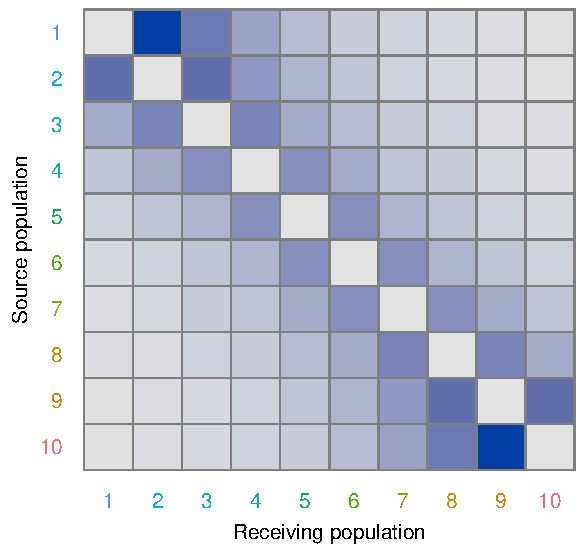
\includegraphics[width=3.5in]{../examples/figure/stray-matrix.pdf}
\caption{An example straying matrix. The rows and columns represent different 
populations (indicated by population number). Dark blue indicates a high rate 
of straying and light blue indicates a low rate of straying.}
\label{f:stray}
\end{figure}

\clearpage

\begin{figure}[htbp]
\centering
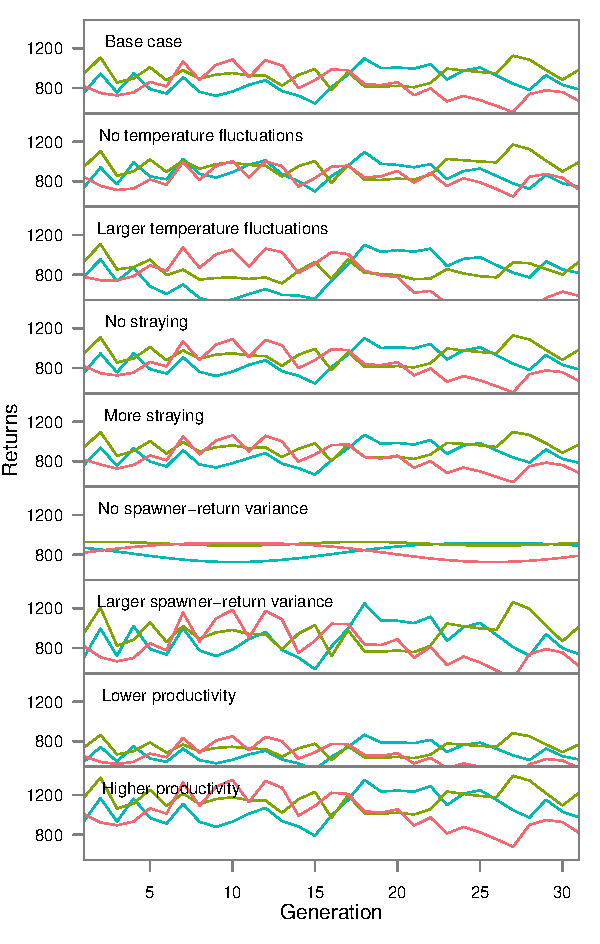
\includegraphics[width=4.0in]{../examples/plot-various-options-ts-3pops.pdf}
\caption{The impact of increasing or decreasing various parameter values on metapopulation return abundance. The different coloured lines represent three example salmon populations. The base case represents the base-case values for the short-term environmental fluctuation scenario.}
\label{f:eg-sens}
\end{figure}

\clearpage

\begin{figure}[htbp]
\centering
\includegraphics[width=4.5in]{../examples/spatial-arma-sim-full.pdf}
\caption{Conserving a \textbf{full range} of response diversity (spatial conservation strategy) with \textbf{short-term} environmental fluctuations.}
\label{f:eg-sp-arma}
\end{figure}

\clearpage

\begin{figure}[htbp]
\centering
\includegraphics[width=4.5in]{../examples/spatial-arma-sim-onehalf.pdf}
\caption{Conserving \textbf{one half} of response diversity (spatial conservation strategy) with \textbf{short-term} environmental fluctuations.}
\label{f:eg-sp-arma}
\end{figure}

\clearpage

\begin{figure}[htbp]
\centering
\includegraphics[width=4.5in]{../examples/spatial-linear-sim-full.pdf}
\caption{Conserving a \textbf{full range} of response diversity (spatial conservation strategy) with \textbf{long-term} environmental fluctuations.}
\label{f:eg-sp-linear}
\end{figure}

\clearpage

\begin{figure}[htbp]
\centering
\includegraphics[width=4.5in]{../examples/spatial-linear-sim-onehalf.pdf}
\caption{Conserving \textbf{one half} of response diversity (spatial conservation strategy) with \textbf{long-term} environmental fluctuations.}
\label{f:eg-sp-linear}
\end{figure}

\clearpage

\begin{figure}[htbp]
\centering
\includegraphics[width=4.5in]{../examples/n-arma-sim-2.pdf}
\caption{\textbf{Two populations} conserved with random response diversity and \textbf{short-term} environmental fluctuations.}
\label{f:eg-n-arma}
\end{figure}

\clearpage

\begin{figure}[htbp]
\centering
\includegraphics[width=4.5in]{../examples/n-arma-sim-16.pdf}
\caption{\textbf{Sixteen populations} conserved with random response diversity and \textbf{short-term} environmental fluctuations.}
\label{f:eg-n-arma}
\end{figure}

\clearpage

\begin{figure}[htbp]
\centering
\includegraphics[width=4.5in]{../examples/n-linear-sim-2.pdf}
\caption{\textbf{Two populations} conserved with random response diversity and \textbf{long-term} environmental change.}
\label{f:eg-n-linear}
\end{figure}

\clearpage

\begin{figure}[htbp]
\centering
\includegraphics[width=4.5in]{../examples/n-linear-sim-16.pdf}
\caption{\textbf{Sixteen populations} conserved with random response diversity and \textbf{long-term} environmental change.}
\label{f:eg-n-linear}
\end{figure}
